\documentclass[./project-report/src/latex/project-report.tex]{subfiles}

\begin{document}

\maketitle

\clearpage
\section{Testing}

\subsection{Investigation}

\subsubsection{test\_model module}
\label{sec:test_model-module}

The test\_model module is contained within the frames package, and contains tkinter frames for testing the trained Artificial Neural Network models for each dataset. 
For each training dataset that an Artificial Neural Network is trained on, there is a corresponding test dataset with completely new images to be tested on to judge 
the performance of the trained model. As fewer images are needed for testing than for training, the Cat dataset only has 50 test images (compared to the 209 images 
for training) and the MNIST dataset only has 10,000 test images (compared to the 60,000 images for training).
Each frame displays the results of the testing along with a random selection of incorrect and correct predictions.

\inputminted{python}{./school_project/frames/test_model.py}

Which outputs the following for the MNIST dataset:

\pagebreak

\begin{figure}[h!]
\centering
\frame{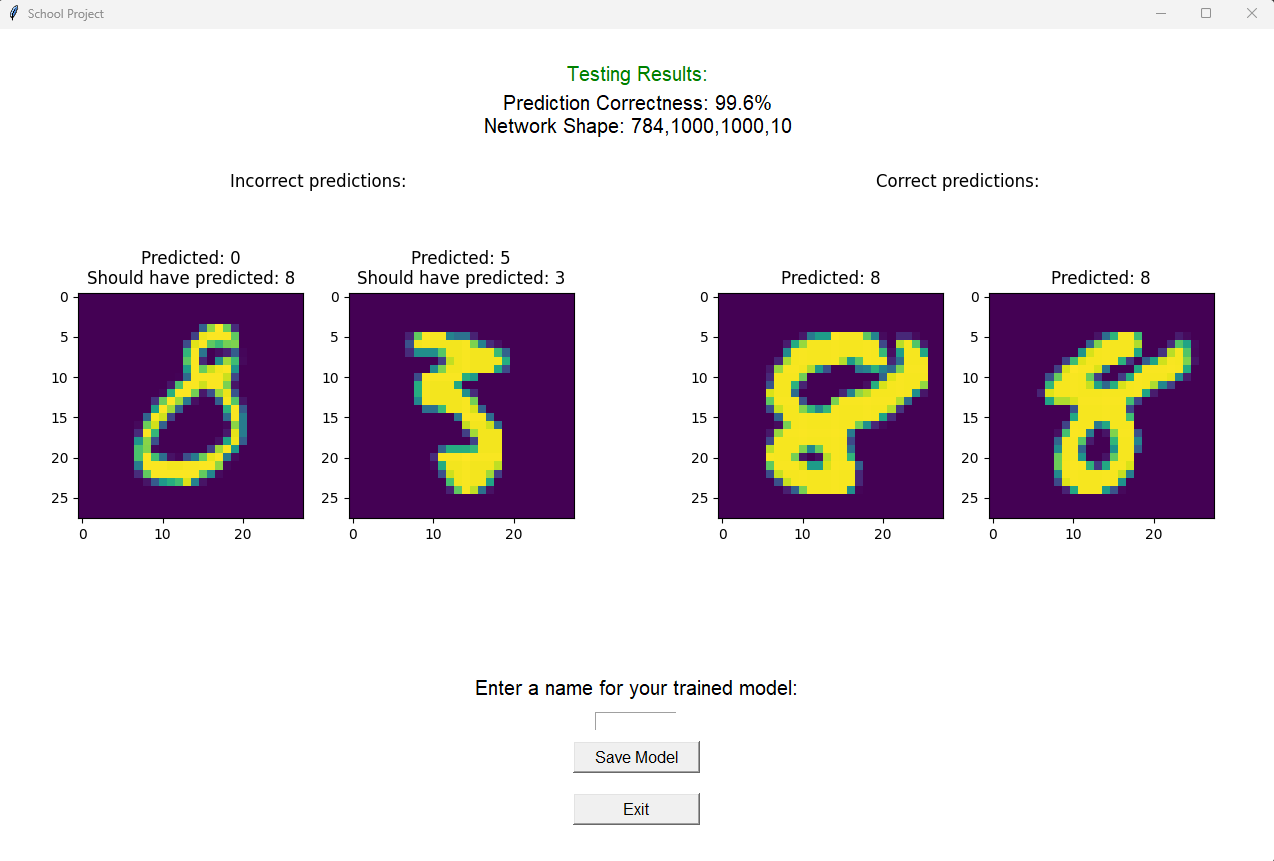
\includegraphics[width=1\textwidth]{./project-report/src/images/test-mnist-frame.png}}
\end{figure}

And outputs the following for the Cat Recognition dataset:

\pagebreak

\begin{figure}[h!]
\centering
\frame{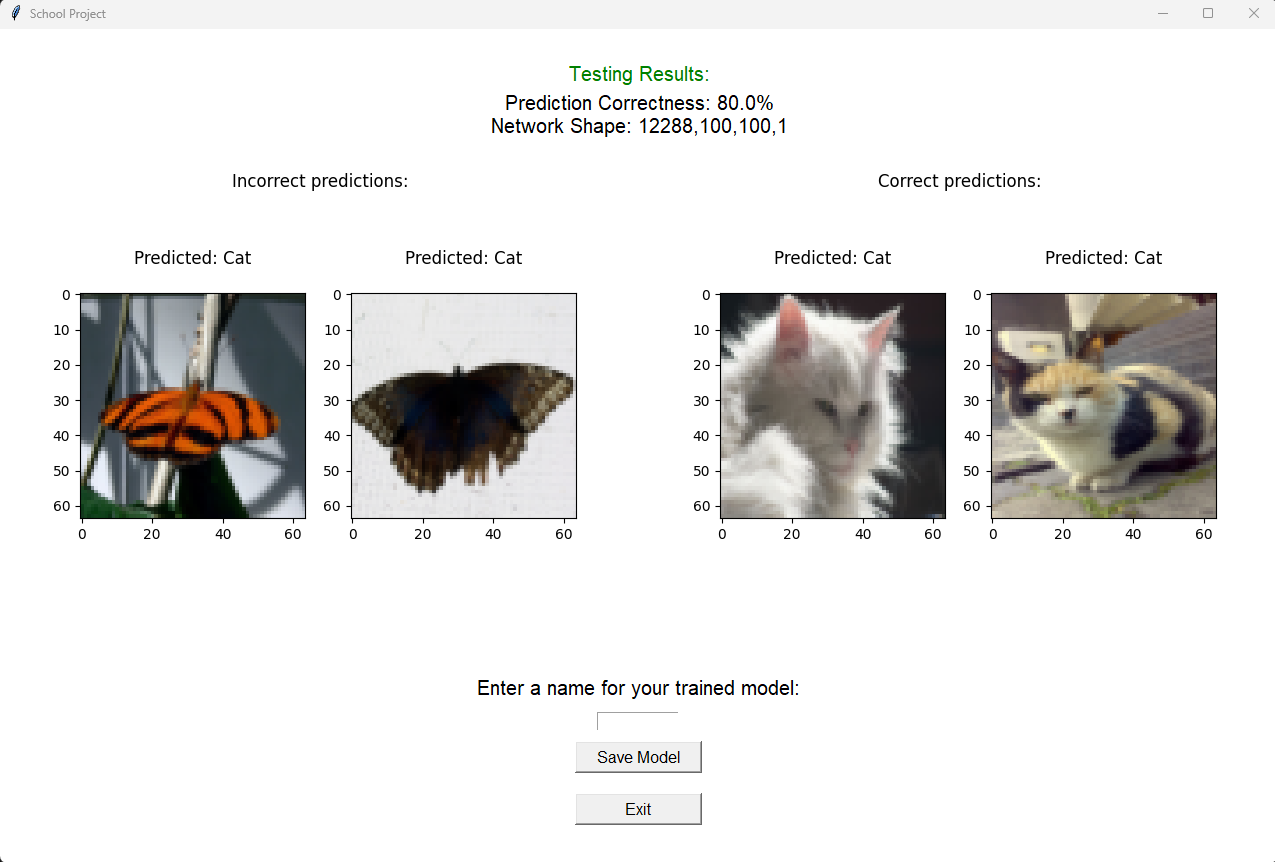
\includegraphics[width=1\textwidth]{./project-report/src/images/test-cat-recognition-frame.png}}
\end{figure}

And outputs the following for the XOR dataset:

\pagebreak

\begin{figure}[h!]
\centering
\frame{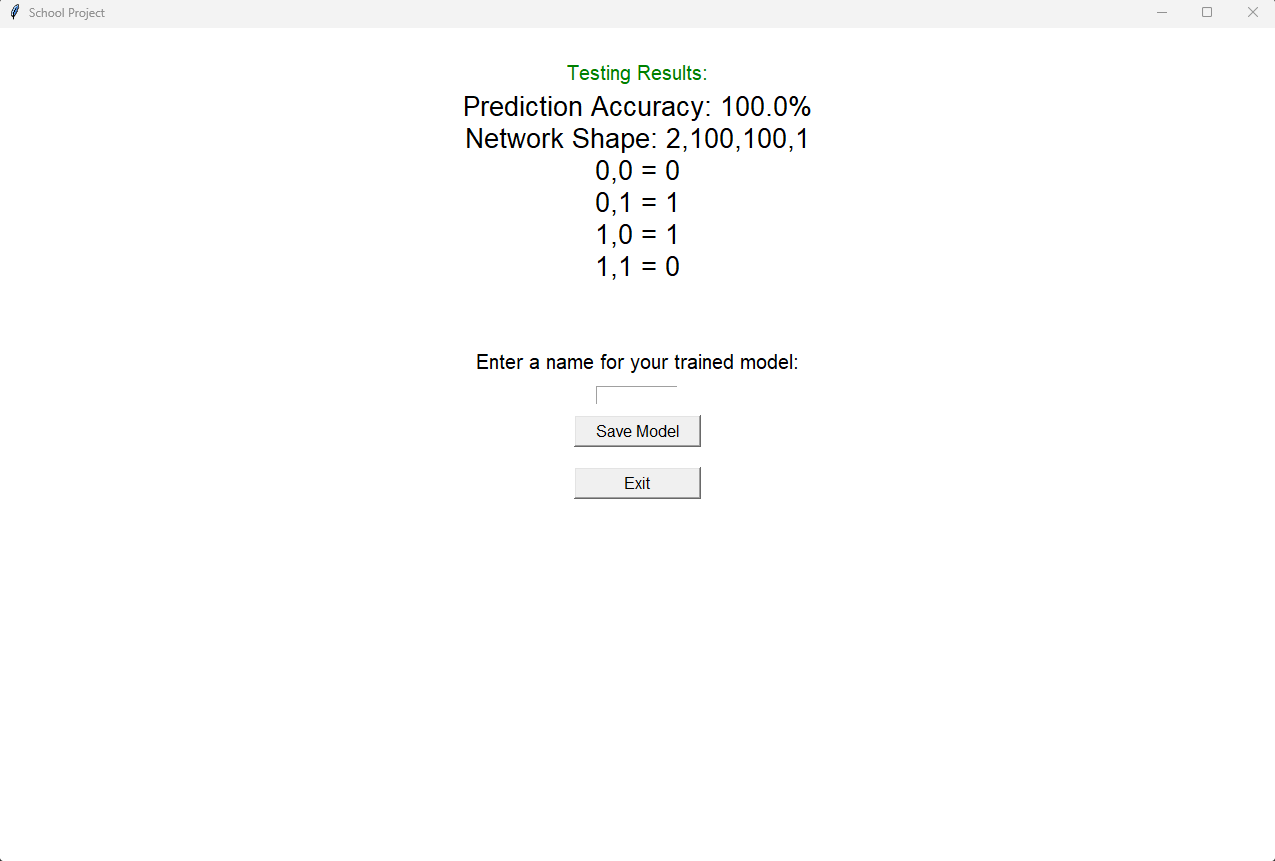
\includegraphics[width=1\textwidth]{./project-report/src/images/test-xor-frame.png}}
\end{figure}

\subsubsection{Effects of Hyper-Parameters}
\label{sec:effects-of-hyper-parameters}

For the following investigations, I utilised Jupyter Notebook and have displayed the results below:

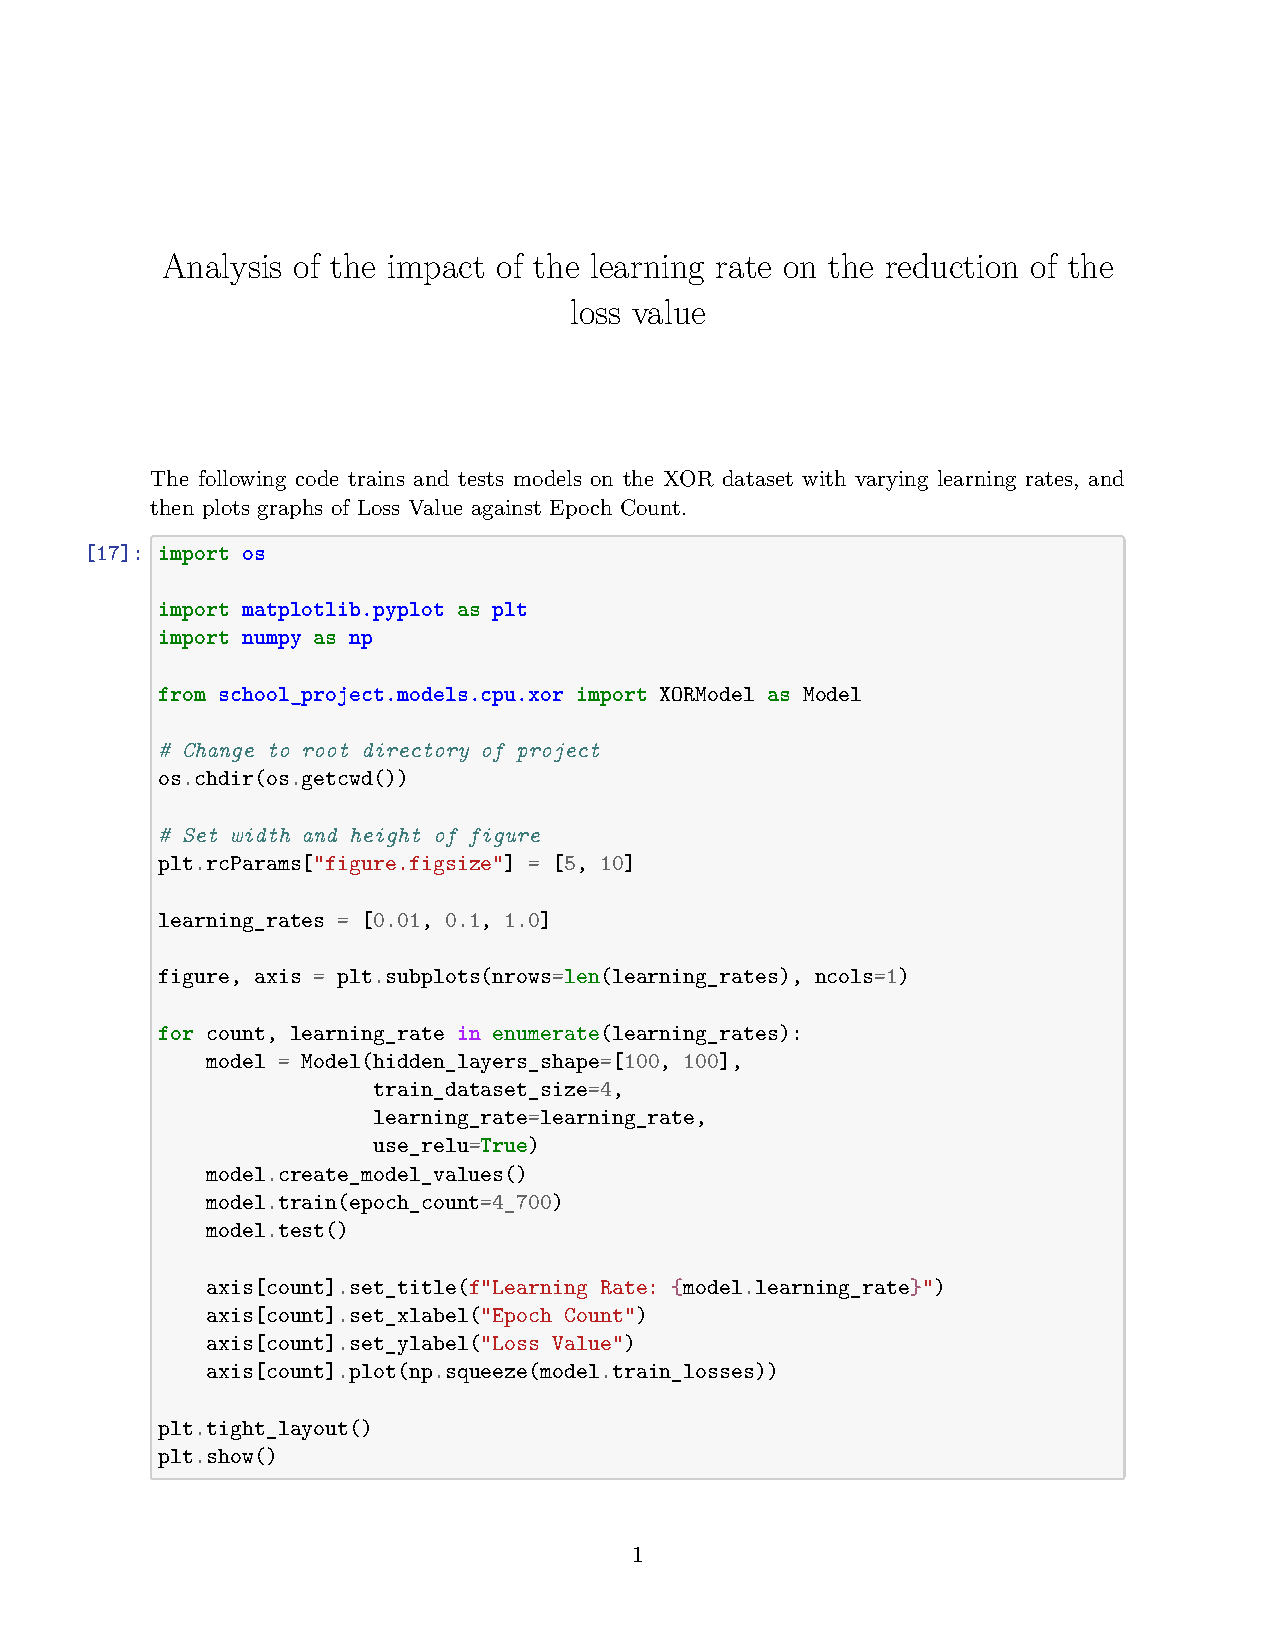
\includepdf[pages=-, pagecommand={\thispagestyle{plain}}, scale=0.9]{./project-report/src/pdfs/learning-rate-analysis.pdf}
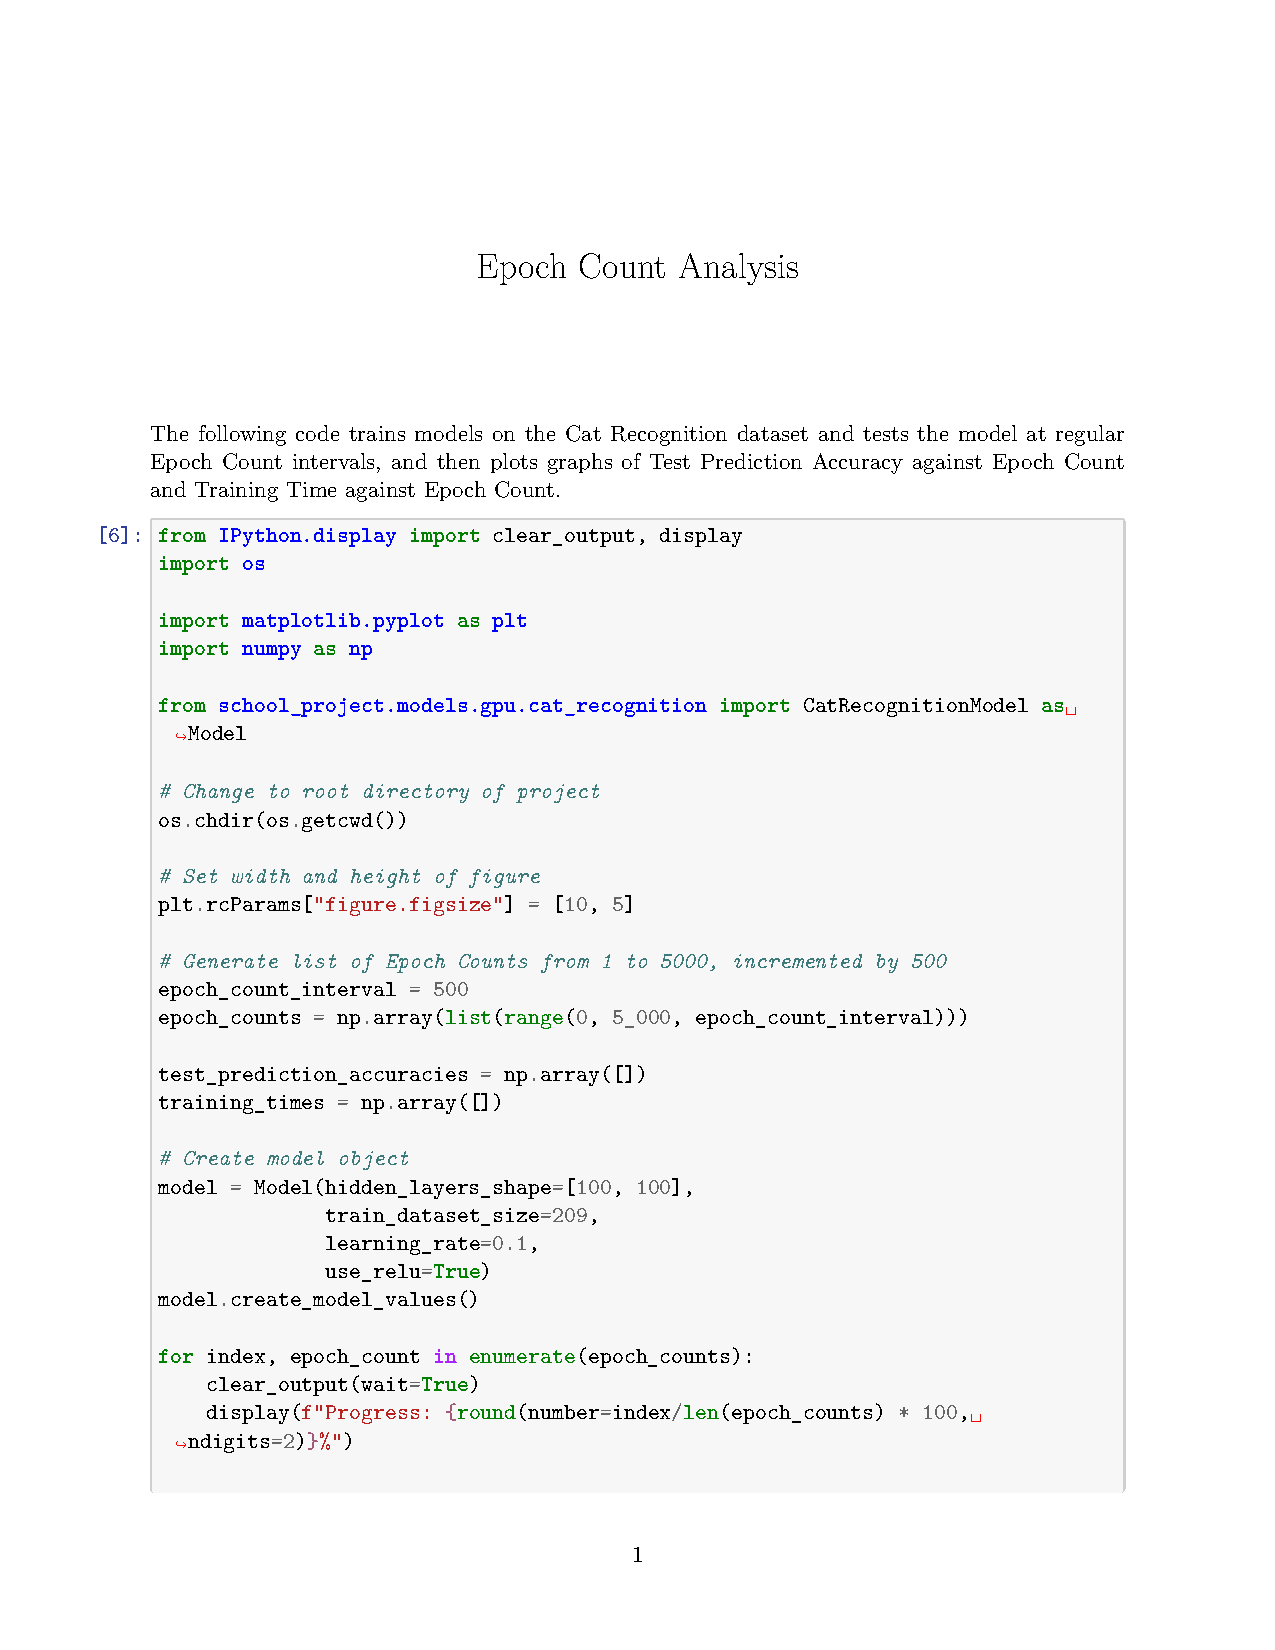
\includepdf[pages=-, pagecommand={\thispagestyle{plain}}, scale=0.9]{./project-report/src/pdfs/epoch-count-analysis.pdf}
\label{sec:train-dataset-size-analysis}
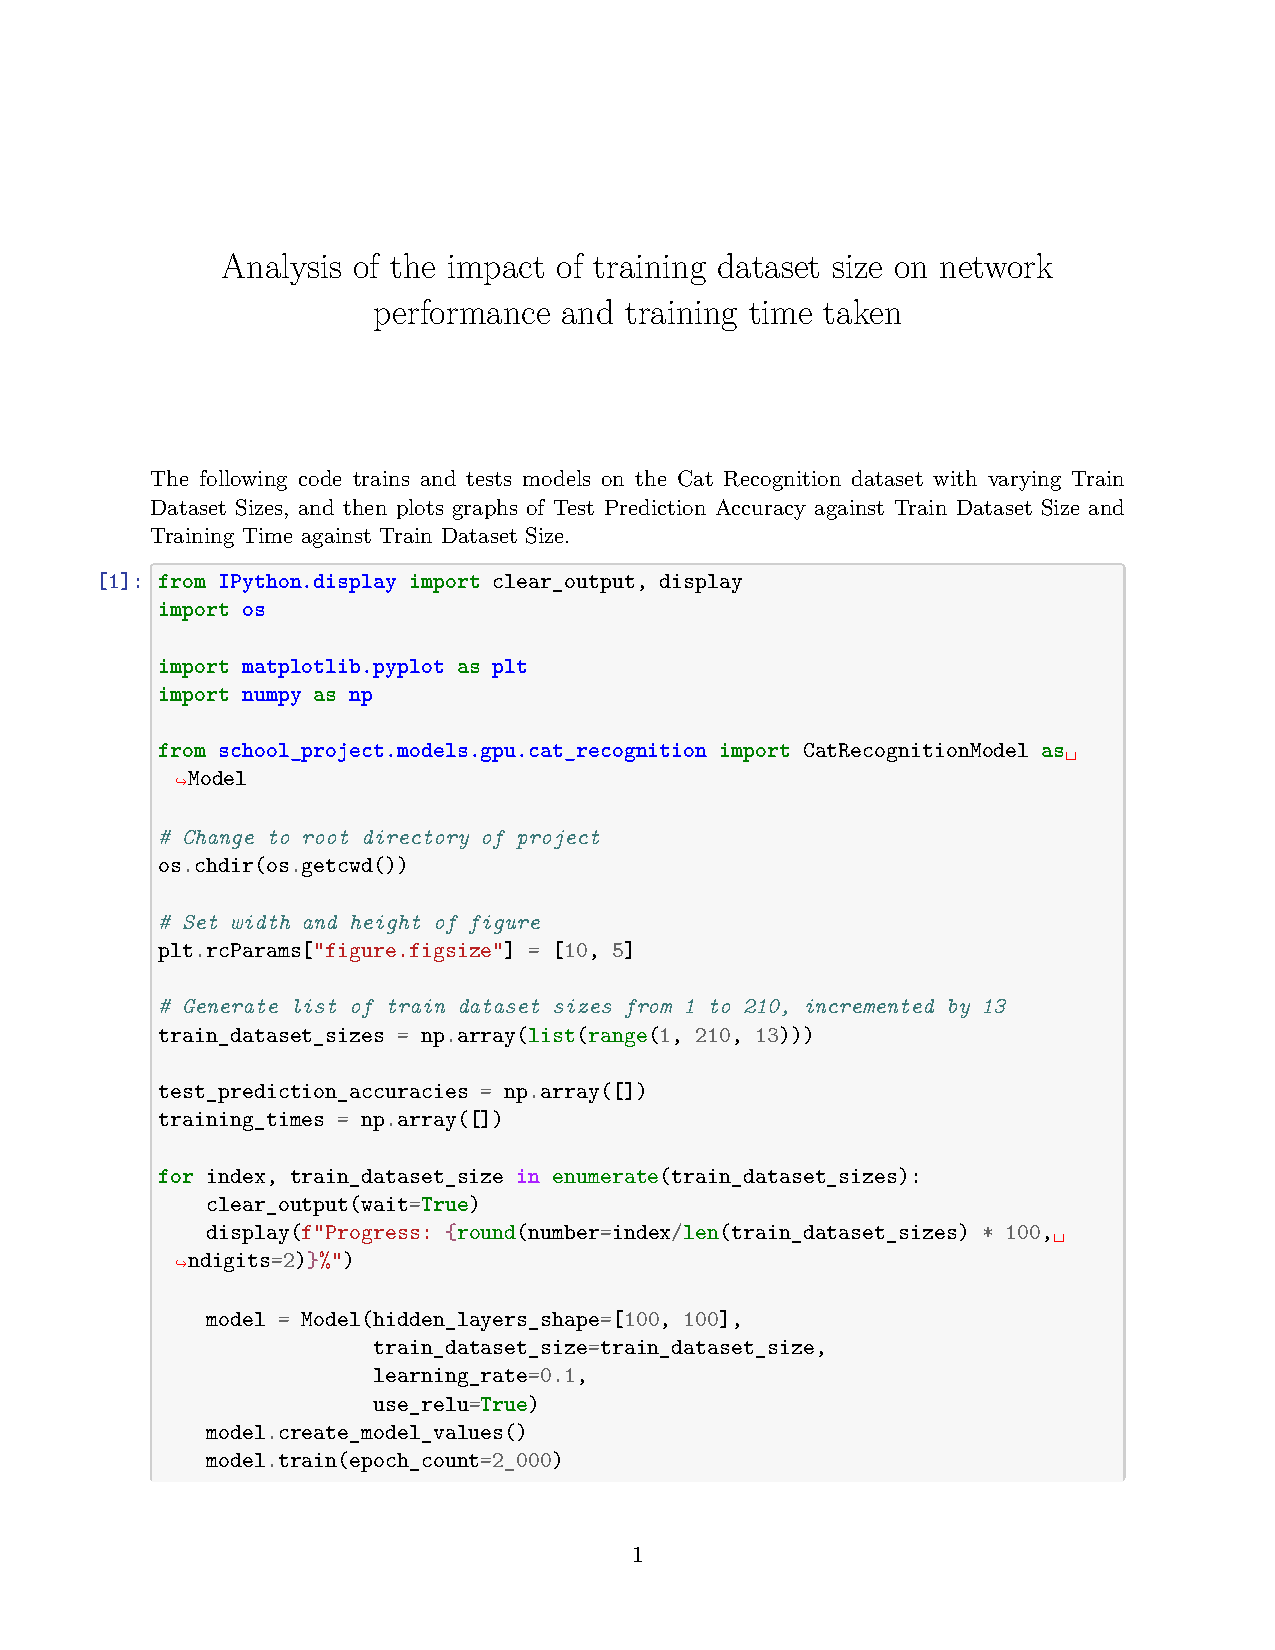
\includepdf[pages=-, pagecommand={\thispagestyle{plain}}, scale=0.9]{./project-report/src/pdfs/train-dataset-size-analysis.pdf}
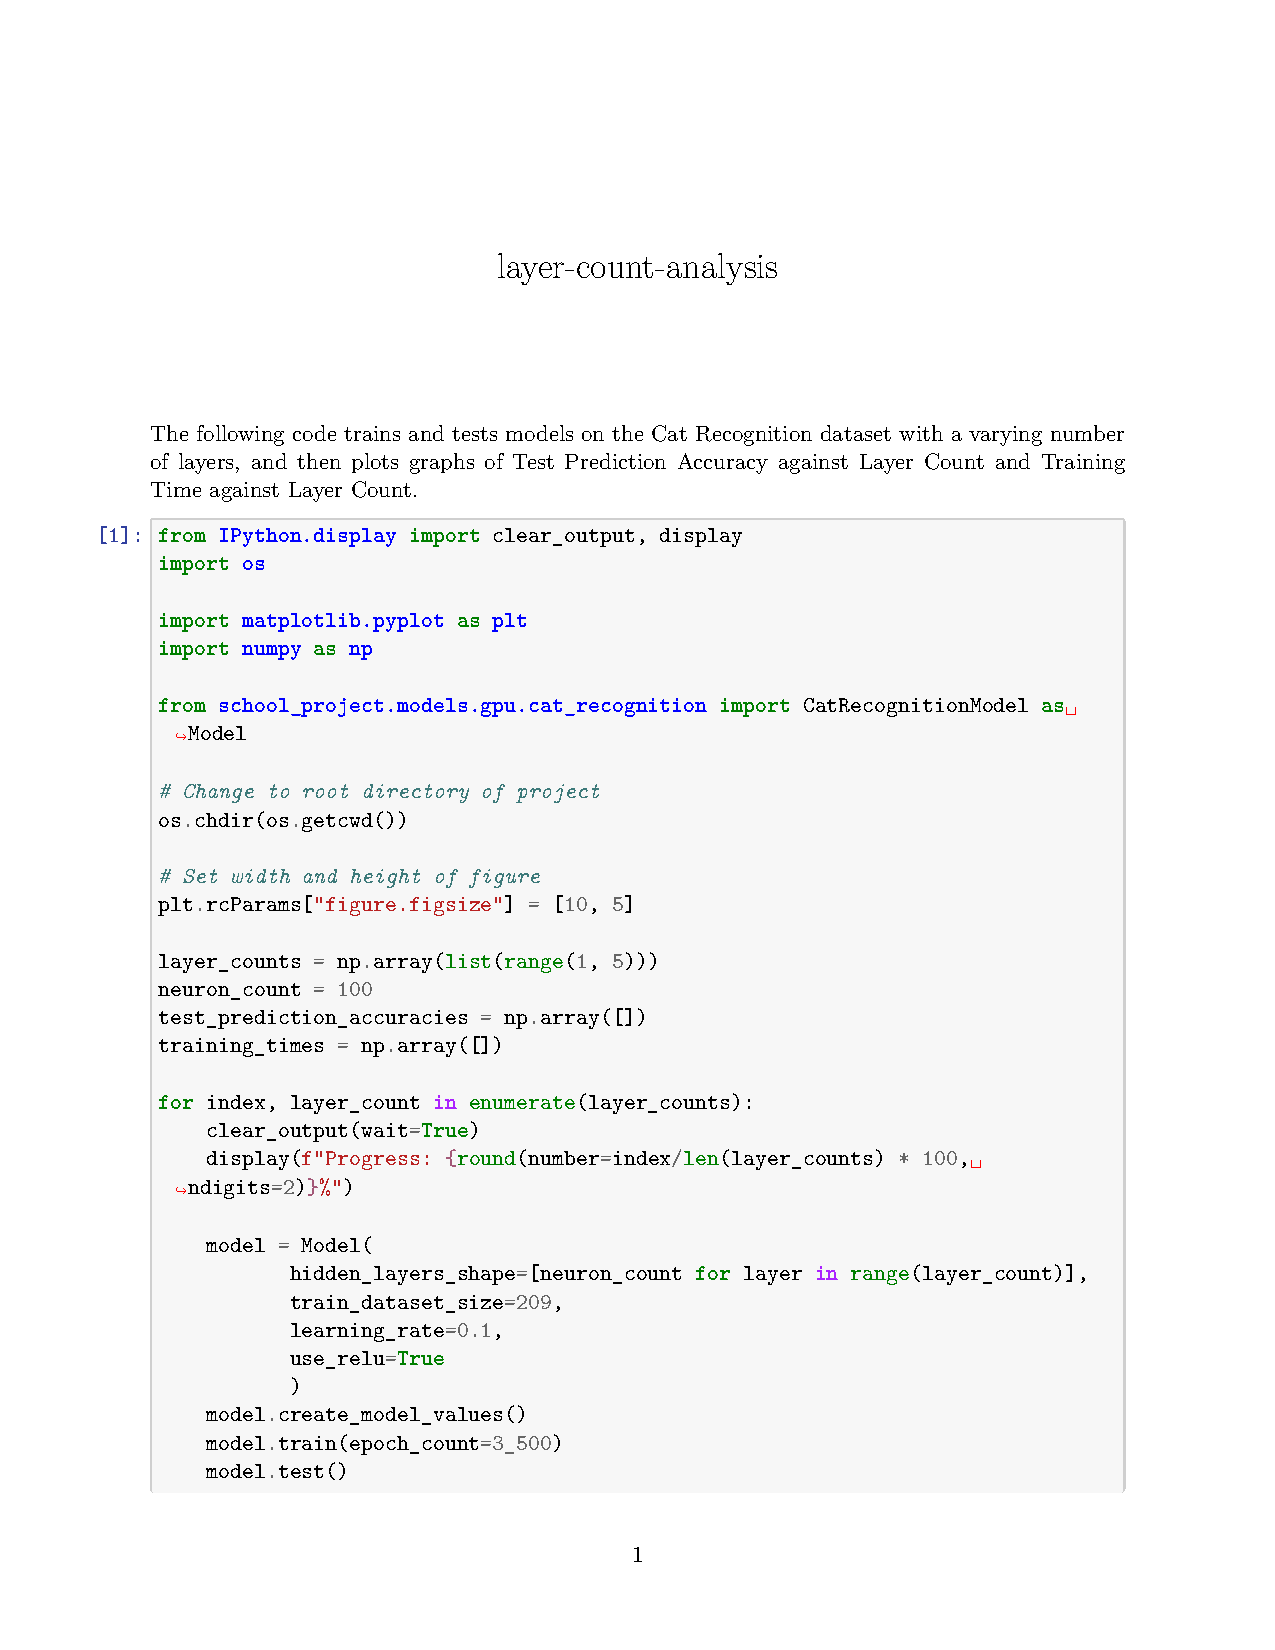
\includepdf[pages=-, pagecommand={\thispagestyle{plain}}, scale=0.9]{./project-report/src/pdfs/layer-count-analysis.pdf}
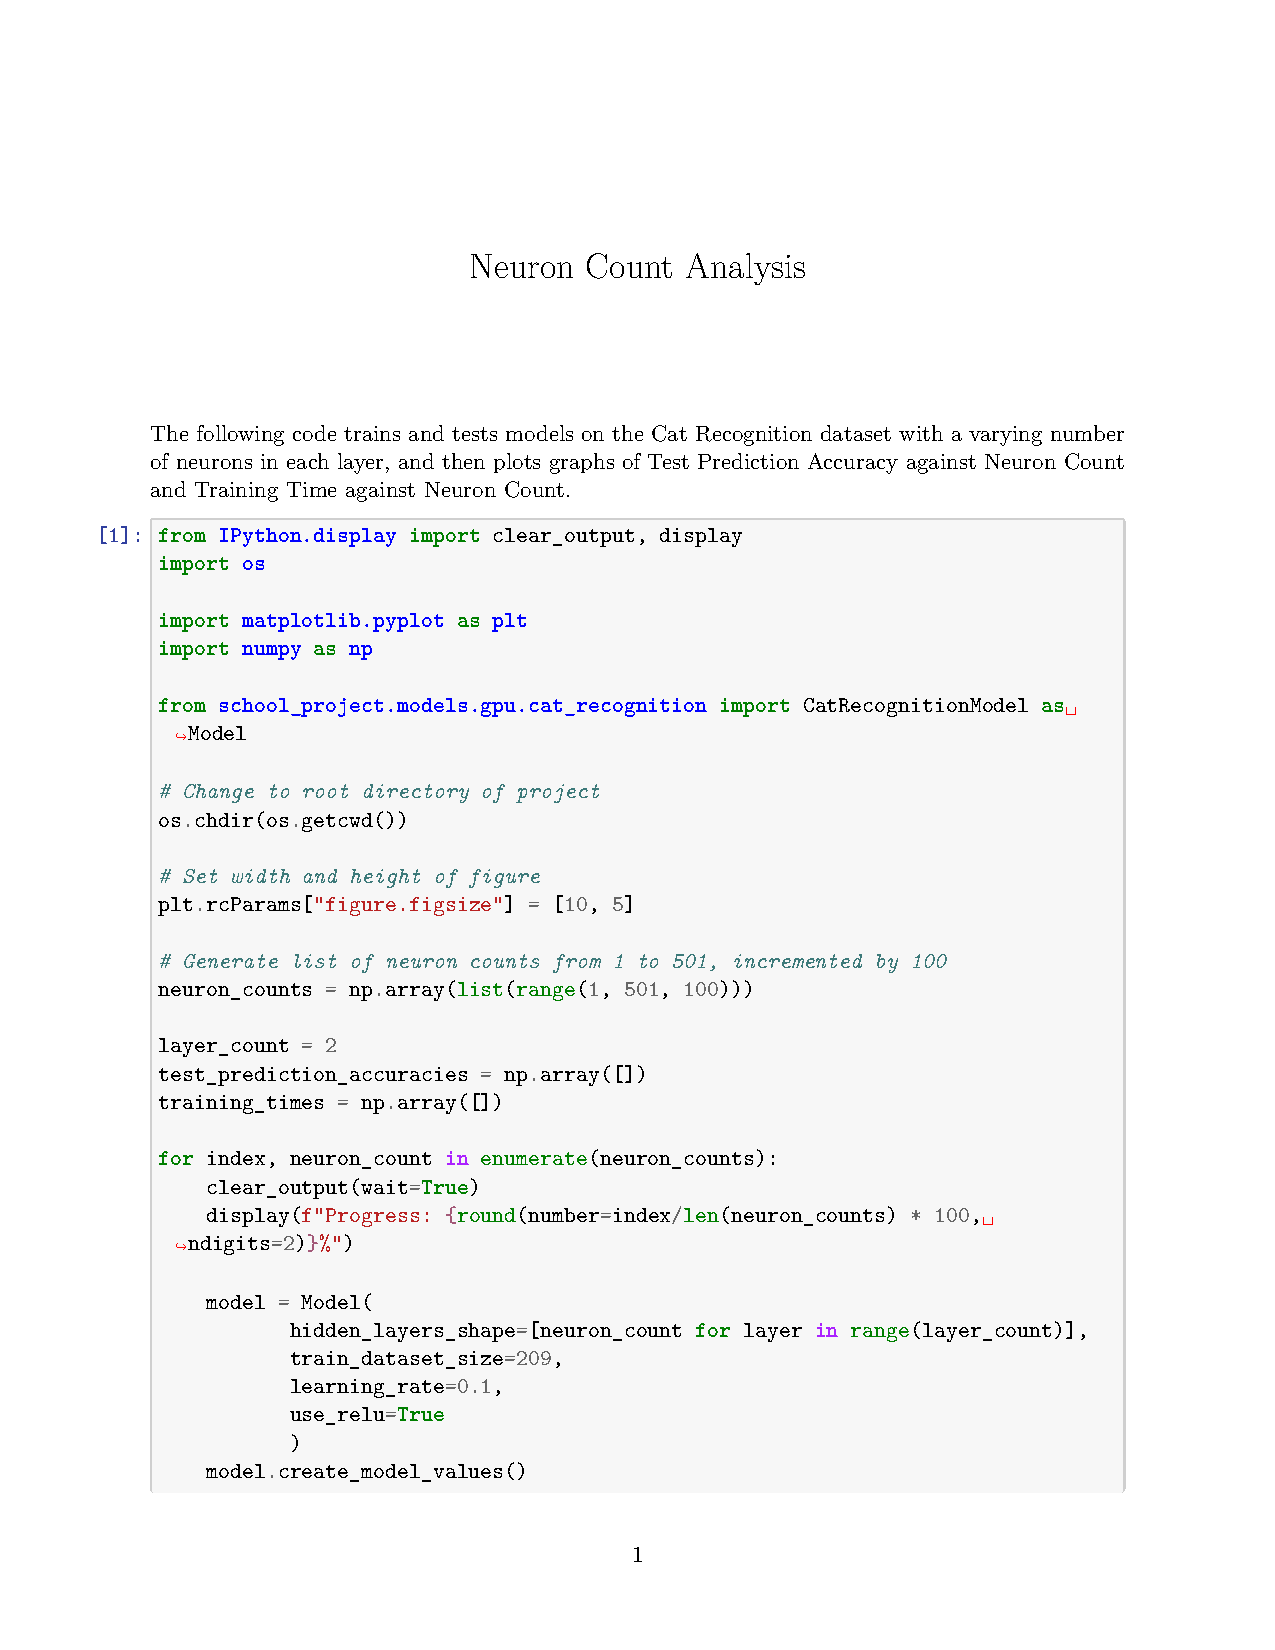
\includepdf[pages=-, pagecommand={\thispagestyle{plain}}, scale=0.9]{./project-report/src/pdfs/neuron-count-analysis.pdf}
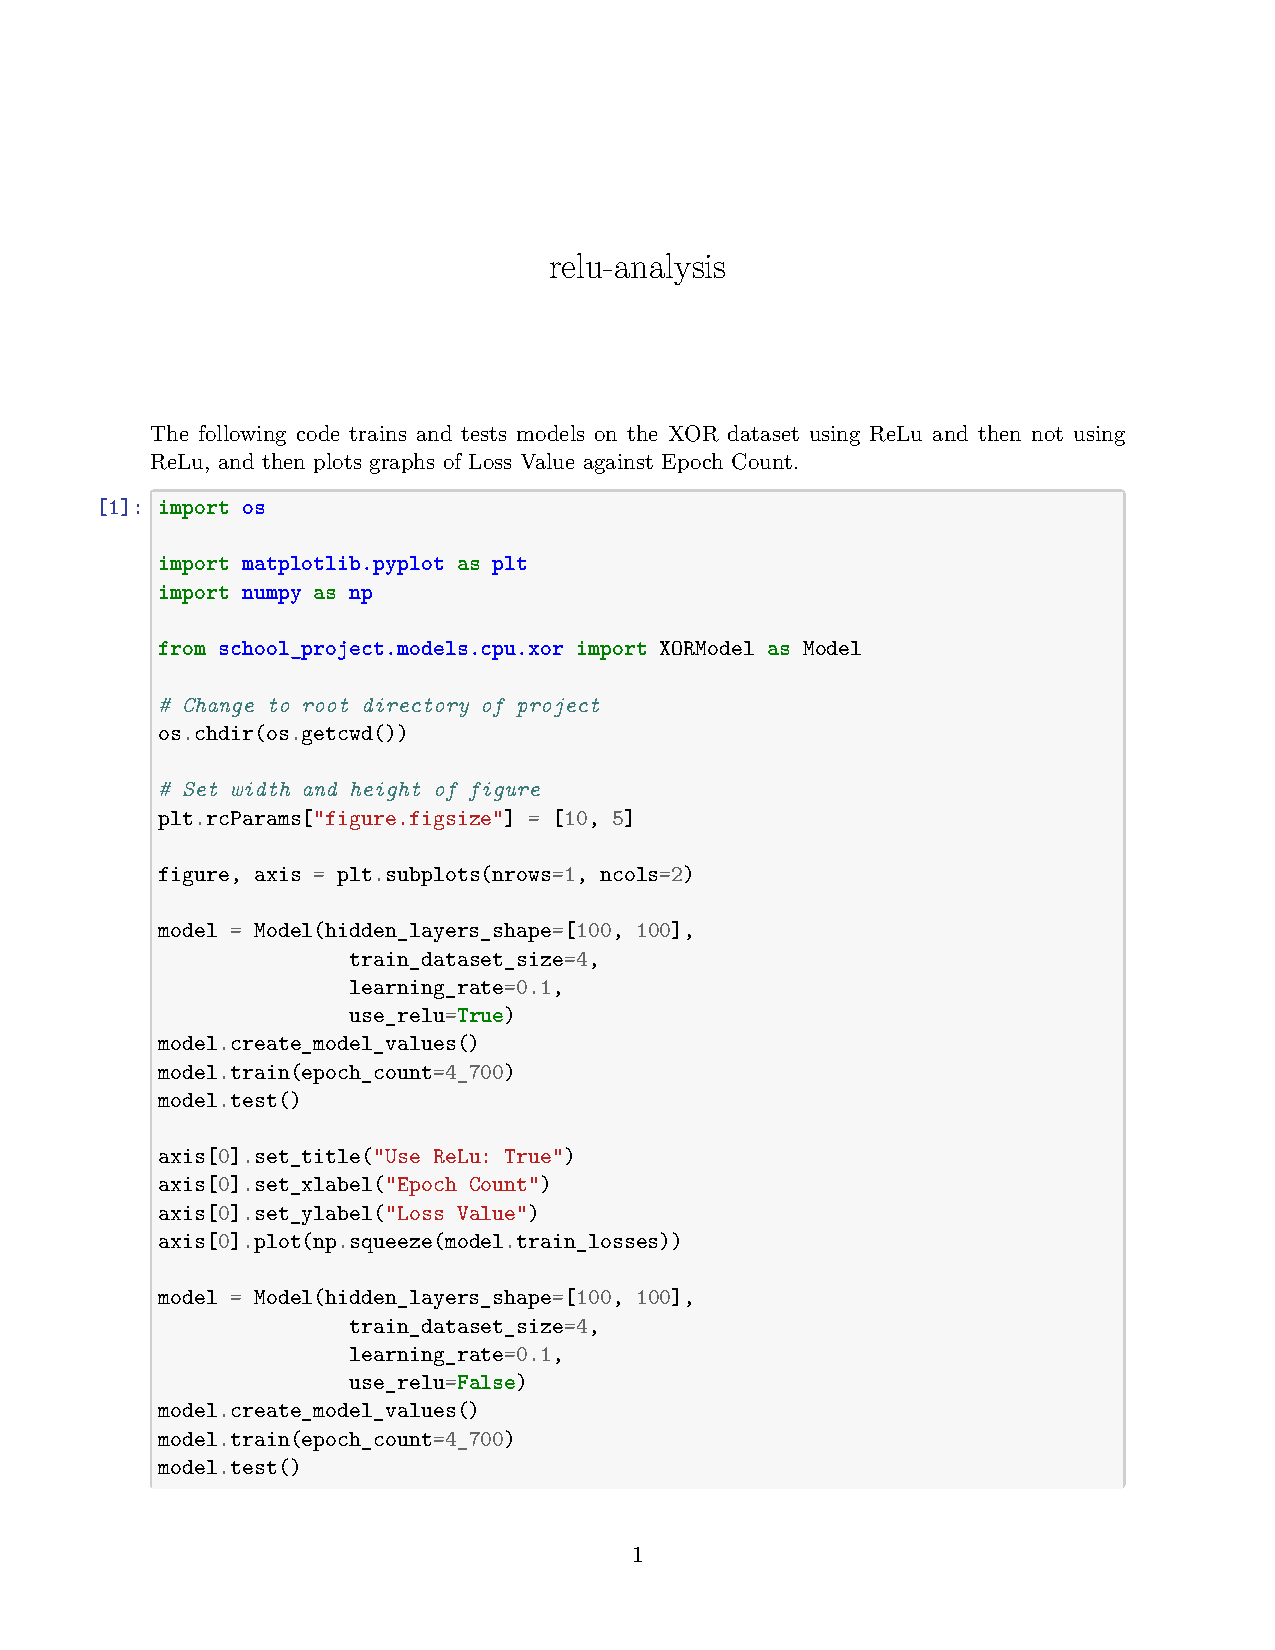
\includepdf[pages=-, pagecommand={\thispagestyle{plain}}, scale=0.9]{./project-report/src/pdfs/relu-analysis.pdf}
\label{sec:cpu-vs-gpu-analysis}
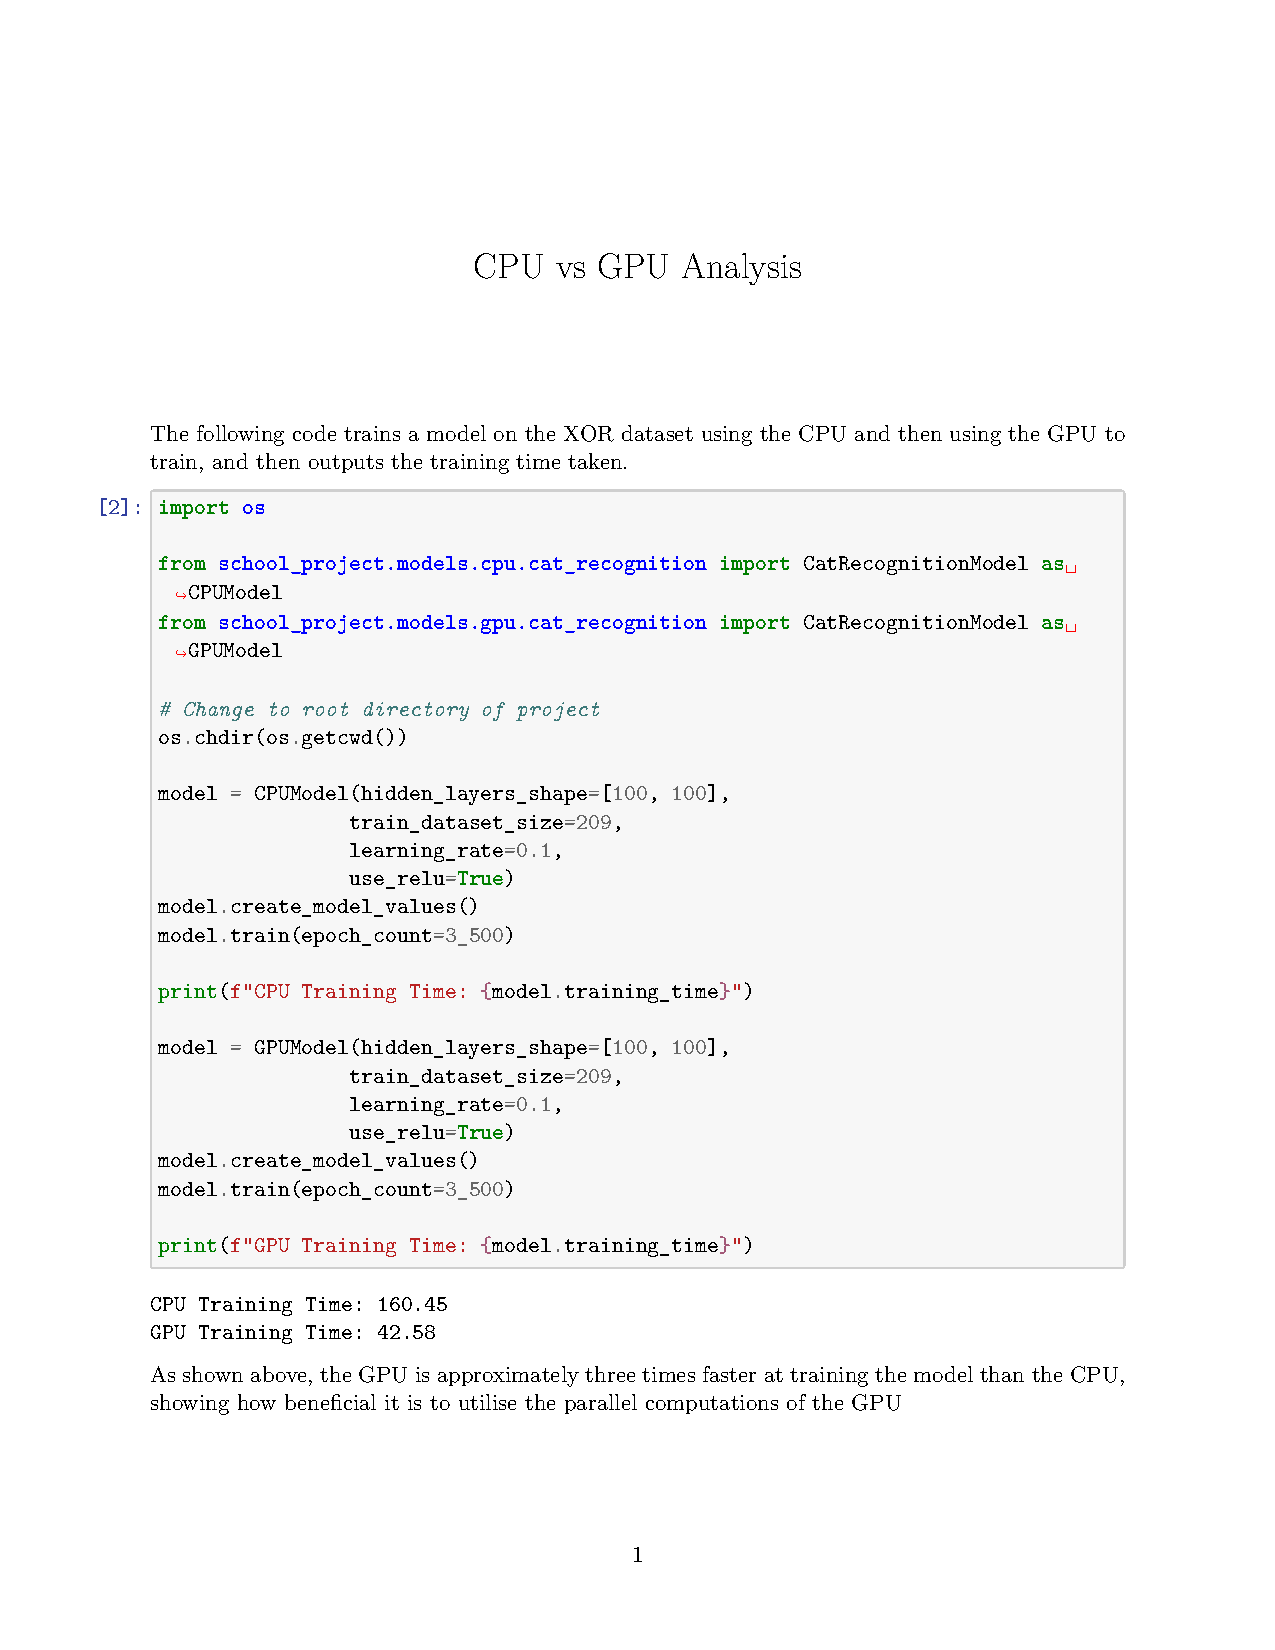
\includepdf[pages=-, pagecommand={\thispagestyle{plain}}, scale=0.9]{./project-report/src/pdfs/cpu-vs-gpu-analysis.pdf}

\subsection{Manual Testing}

\subsubsection{Input Validation Testing} % See table on teams

The following tests check the input validation of each frames' inputs.

\begin{itemize}
    \item Hyper Parameter Frame:
    \label{sec:hyper-parameter-frame-input-validation}
    \begin{itemize}
        \item Use GPU Validation:
            \begin{itemize}
                \item Description: Select Use GPU checkbox without a GPU present.
                \item Expected Result: The exception should be handled and a useful error message should be displayed.
                \item Actual Result: Expected Result
                \item Test Status: Pass
                \item Evidence:
                    \begin{figure}[h!]
                    \centering
                    \frame{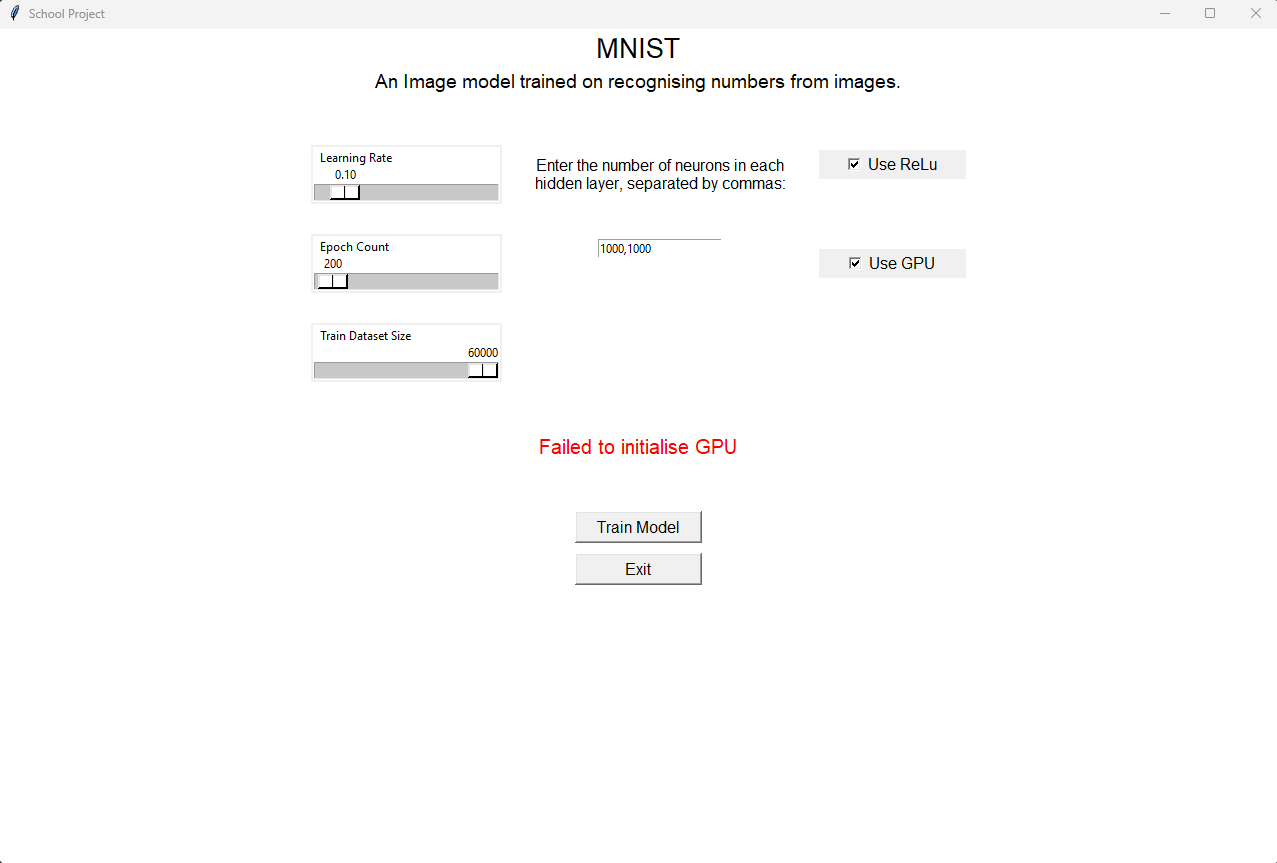
\includegraphics[width=1\textwidth]{./project-report/src/images/create-model-use-gpu-validation.png}}
                    \end{figure}

                    Link to video evidence: \url{https://github.com/mcttn22/school-project/blob/main/project-report/input-validation-testing-videos.md/#use-gpu-validation}
            \end{itemize}

        \pagebreak

        \item Hidden Layers Shape Validation:
            \begin{itemize}
                \item Description: Enter an invalid hidden layers shape.
                \item Data Value: "test"
                \item Data Type: Erroneous
                \item Expected Result: The exception should be handled and a useful error message should be displayed.
                \item Actual Result: Expected Result
                \item Test Status: Pass
                \item Evidence:
                    \begin{figure}[h!]
                    \centering
                    \frame{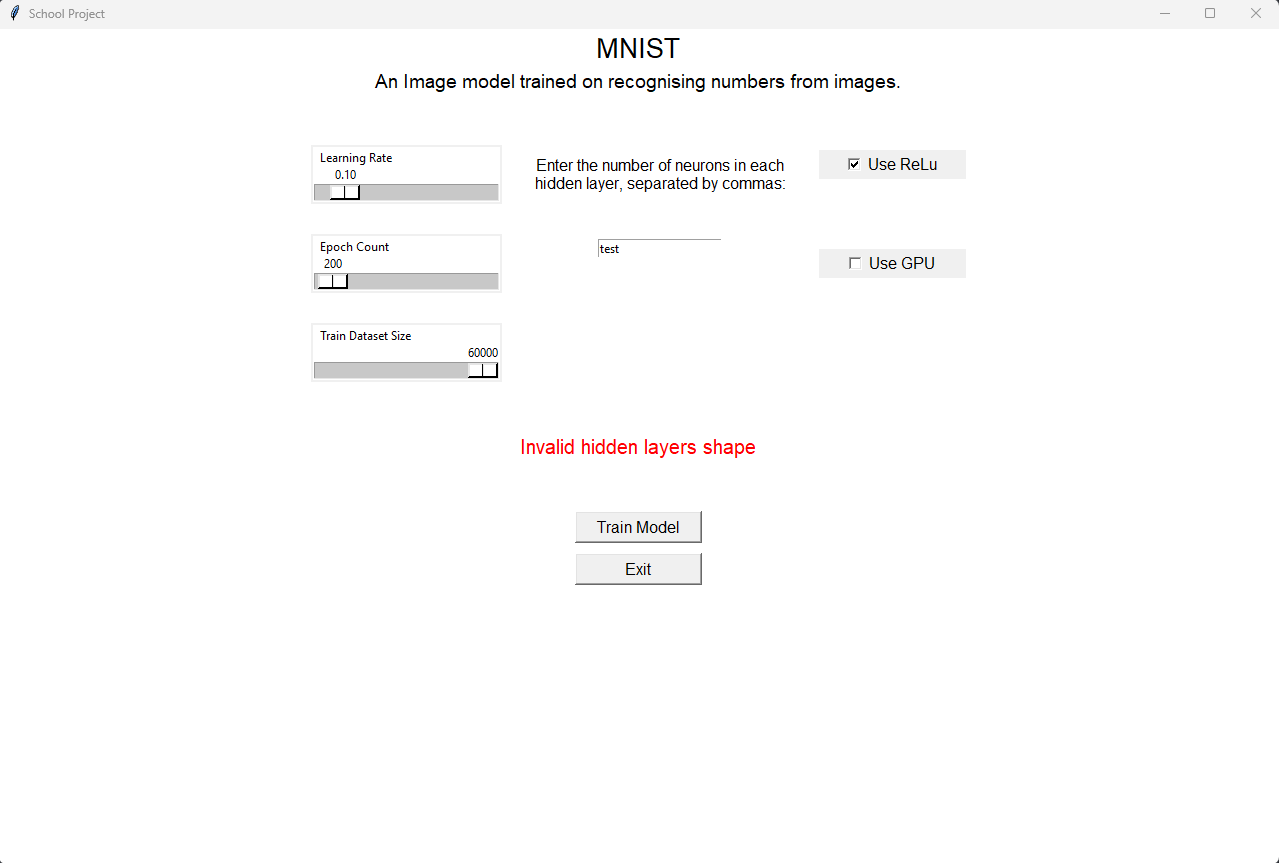
\includegraphics[width=1\textwidth]{./project-report/src/images/hidden-layers-shape-input-validation.png}}
                    \end{figure}

                    Link to video evidence: \url{https://github.com/mcttn22/school-project/blob/main/project-report/input-validation-testing-videos.md/#hidden-layers-shape-validation}
            \end{itemize}
    \end{itemize}

    \pagebreak

    \item Load Model Frame:
    \label{sec:load-model-frame-input-validation}
    \begin{itemize}
        \item Use GPU Validation:
            \begin{itemize}
            \item Description: Select Use GPU checkbox without a GPU present.
            \item Expected Result: The exception should be handled and a useful error message should be displayed.
            \item Actual Result: Expected Result
            \item Test Status: Pass
            \item Evidence:
                \begin{figure}[h!]
                \centering
                \frame{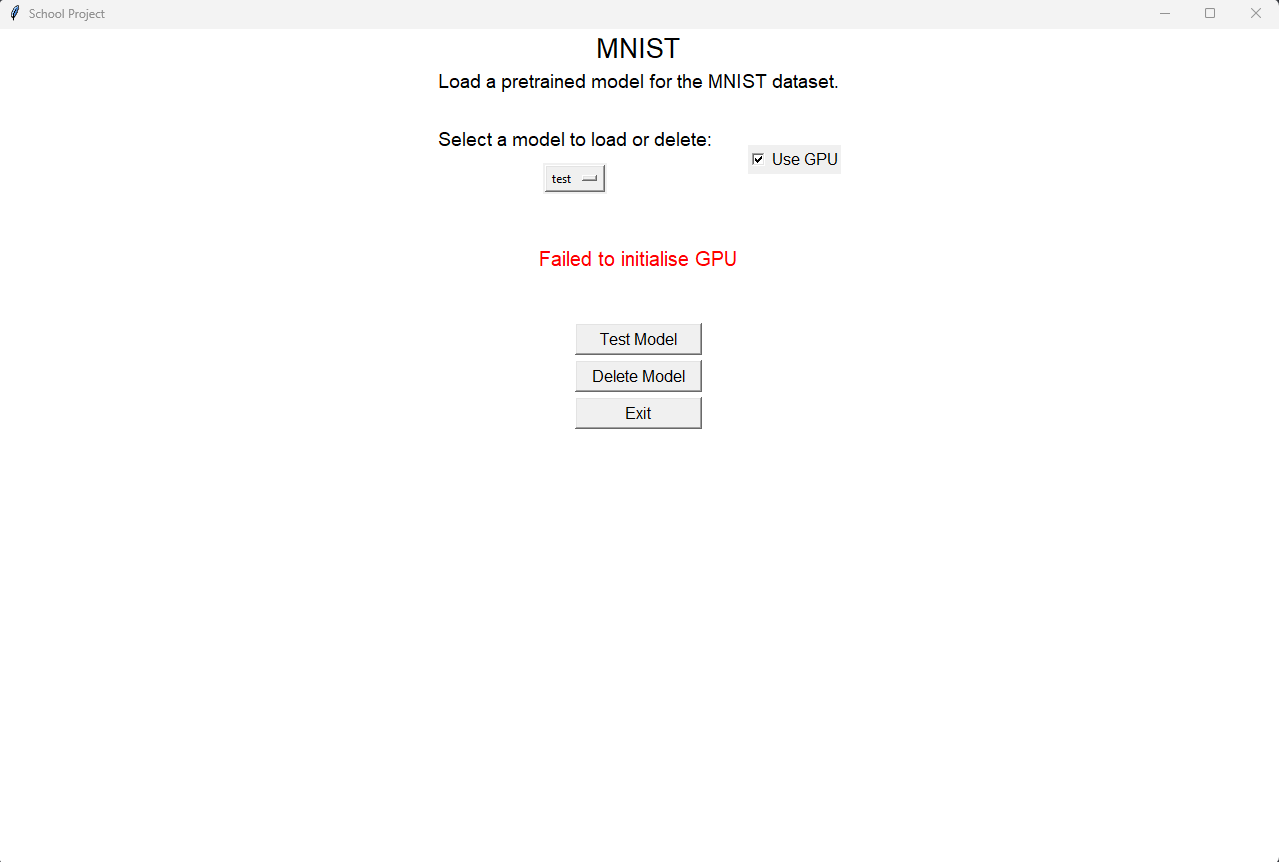
\includegraphics[width=1\textwidth]{./project-report/src/images/load-model-use-gpu-validation.png}}
                \end{figure}

                Link to video evidence: \url{https://github.com/mcttn22/school-project/blob/main/project-report/input-validation-testing-videos.md/#hidden-layers-shape-validation}
            \end{itemize}
    \end{itemize}

    \pagebreak

    \item Test Frames:
    \label{sec:test-frames-input-validation}
    \begin{itemize}
        \item Taken Trained Model Name Validation:
            \begin{itemize}
                \item Description: Try to save a trained model with an already taken name.
                \item Data Value: "test"
                \item Data Type: Erroneous
                \item Expected Result: The exception should be handled and a useful error message should be displayed.
                \item Actual Result: Expected Result
                \item Test Status: Pass
                \item Evidence:
                    \begin{figure}[h!]
                    \centering
                    \frame{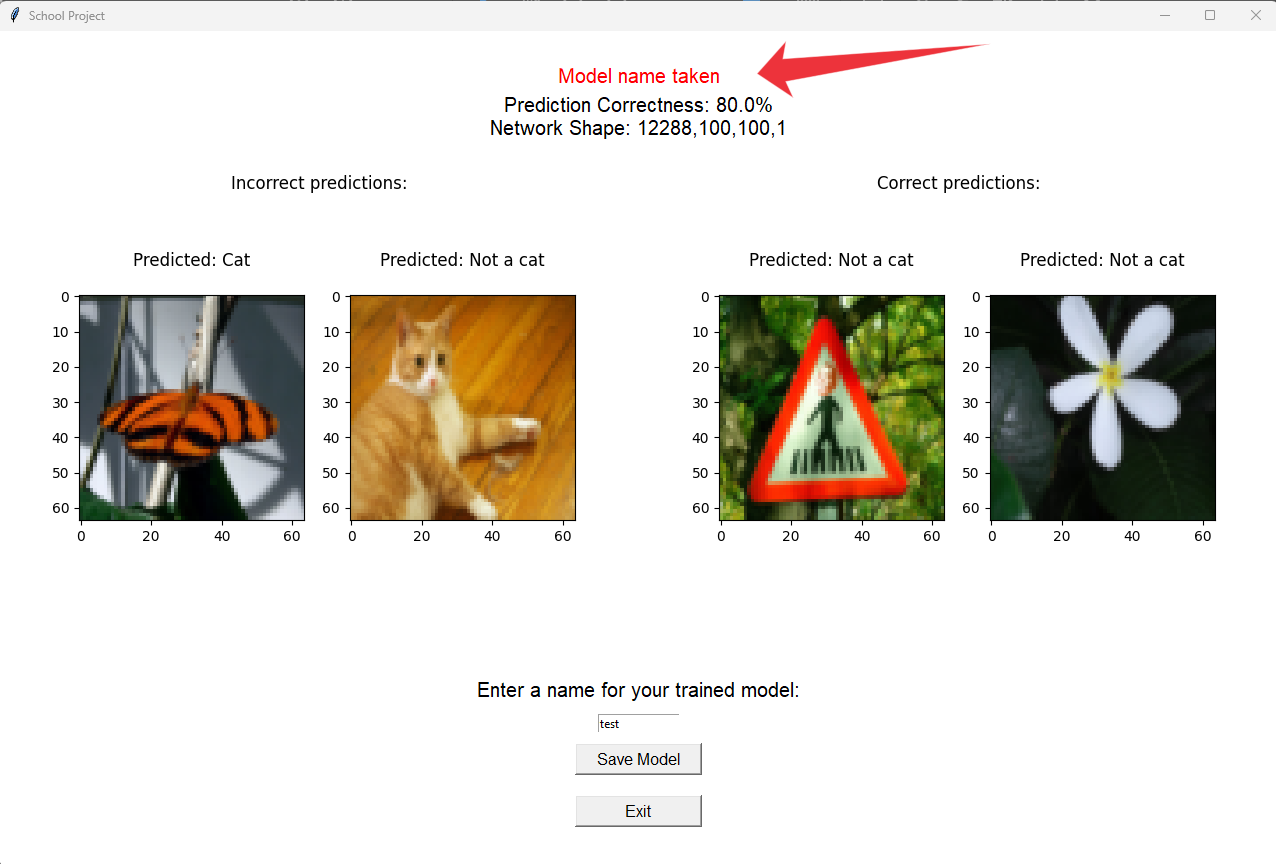
\includegraphics[width=1\textwidth]{./project-report/src/images/taken-trained-model-name-input-validation.png}}
                    \end{figure}

                    Link to video evidence: \url{https://github.com/mcttn22/school-project/blob/main/project-report/input-validation-testing-videos.md/#hidden-layers-shape-validation}
            \end{itemize}

        \pagebreak
        
        \item Empty Trained Model Name Validation:
            \begin{itemize}
                \item Description: Try to save a trained model with blank name.
                \item Data Value: ""
                \item Data Type: Erroneous
                \item Expected Result: The exception should be handled and a useful error message should be displayed.
                \item Actual Result: Expected Result
                \item Test Status: Pass
                \item Evidence:
                    \begin{figure}[h!]
                    \centering
                    \frame{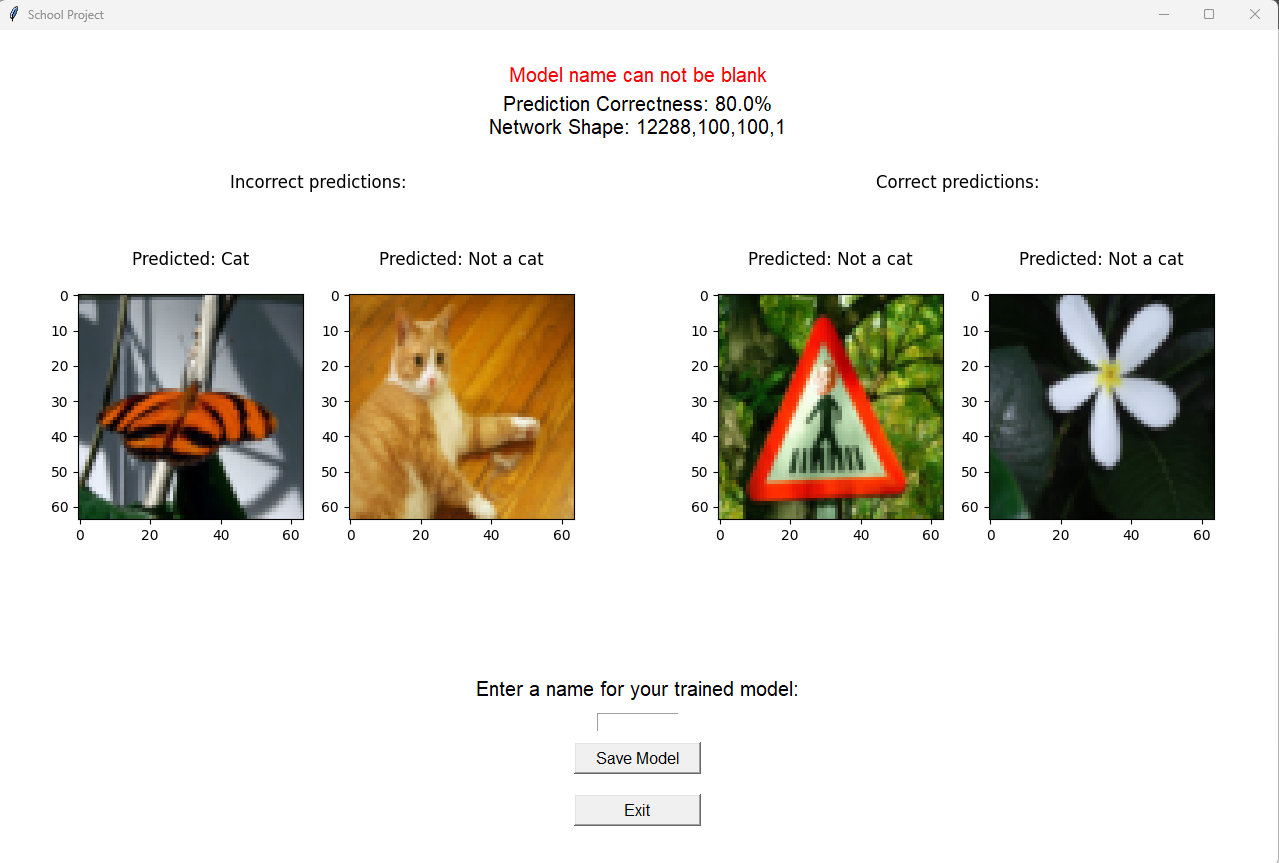
\includegraphics[width=1\textwidth]{./project-report/src/images/empty-trained-model-name-input-validation.png}}
                    \end{figure}

                    Link to video evidence: \url{https://github.com/mcttn22/school-project/blob/main/project-report/input-validation-testing-videos.md/#hidden-layers-shape-validation}
            \end{itemize}
    \end{itemize}
\end{itemize}

\subsection{Automated Testing}

\subsubsection{Unit Tests}

Within the test package, I have written the following unit tests:

\begin{itemize}
    \label{sec:database-unit-tests}
    \item Unit tests for the database in a test\_database.py module:
        \begin{itemize}
            \item test\_database\_structure:
            \begin{itemize}
                \item Description: Test that the database tables are set up correctly.
                \item Expected Result: Check that the 'Models' table exists in the database and that the table's info matches the following format: \newline
                [(0, 'Model\_ID', 'INTEGER', 0, None, 1), \newline
                (1, 'Dataset', 'TEXT', 1, None, 0), \newline
                (2, 'File\_Location', 'TEXT', 1, None, 0), \newline
                (3, 'Hidden\_Layers\_Shape', 'TEXT', 1, None, 0), \newline
                (4, 'Learning\_Rate', 'FLOAT', 1, None, 0), \newline
                (5, 'Name', 'TEXT', 1, None, 0), \newline
                (6, 'Train\_Dataset\_Size', 'INTEGER', 1, None, 0), \newline
                (7, 'Use\_ReLu', 'INTEGER', 1, None, 0)]
                \item Actual Result: Expected Result
                \item Test Status: Pass
            \end{itemize}
			\item test\_not\_null\_constraint:
			\begin{itemize}
				\item Description: Test that the NOT NULL constraint is setup.
				\item Data Value: \newline
					 ("Test\_Dataset", \newline
                     f"school\_project/saved-models/{uuid.uuid4().hex}.npz", \newline
                     "100, 100", \newline
                     0.1, \newline
                     "Test\_Name", \newline
                     100)
				\item Data Type: Erroneous
				\item Expected Result: A sqlite3.IntegrityError should be raised.
				\item Actual Result: Expected Result
				\item Test Status: Pass
			\end{itemize}
			\item test\_unique\_constraint:
			\begin{itemize}
				\item Description: Test that the UNIQUE (Dataset, Name) constraint is setup.
				\item Data Value: \newline
					  ("Test\_Dataset", \newline
                     f"school\_project/saved-models/{uuid.uuid4().hex}.npz", \newline
                     "100, 100", \newline
                     0.1, \newline
                     "Test\_Name", \newline
                     100, \newline
                     True)
				\item Data Type: Erroneous
				\item Expected Result: A sqlite3.IntegrityError should be raised.
				\item Actual Result: Expected Result
				\item Test Status: Pass
			\end{itemize}
			\item test\_save\_load\_consistency:
			\begin{itemize}
				\item Description: Test that data is not changed between saving and loading.
				\item Data Value: \newline
					  ("Test\_Dataset", \newline
                      f"school\_project/saved-models/{uuid.uuid4().hex}.npz", \newline
                      "100, 100", \newline
                      0.1, \newline
                      "Test\_Name", \newline
                      100, \newline
                      True)
				\item Data Type: Normal
				\item Expected Result: Data is not changed between saving and loading.
				\item Actual Result: Expected Result
				\item Test Status: Pass
			\end{itemize}
            \item Evidence:
                \inputminted{python}{./school_project/test/test_database.py}

				\pagebreak

				\begin{figure}[h!]
				\centering
				\frame{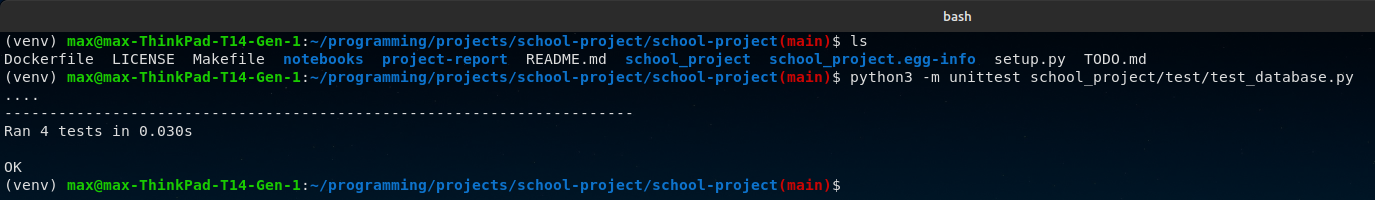
\includegraphics[width=1\textwidth]{./project-report/src/images/test-database.png}}
				\end{figure}

				Link to video evidence: \url{https://github.com/mcttn22/school-project/blob/main/project-report/input-validation-testing-videos.md/#test_databasepy}
		\end{itemize}
    
    \label{sec:models-utils-unit-tests}
    \item Unit tests for the utils subpackage of both the cpu and gpu subpackage of the models package. Similarly to the code for the cpu and gpu subpackage, it is 
          only worth showing the code for the cpu version as both are very similar in functionality.
        \begin{itemize}
            \item test\_model.py module:
				\begin{itemize}
					\item test\_train\_dataset\_size:
					\begin{itemize}
						\item Description: Test the size of training dataset to be value chosen.
						\item Data Value: \newline
							hidden\_layers\_shape = [100, 100], \newline
                         	train\_dataset\_size = 4, \newline
                         	learning\_rate = 0.1, \newline
                         	use\_relu = True
						\item Data Type: Normal
						\item Expected Result: The number of columns of the training input matrix should be equal to 4.
						\item Actual Result: Expected Result
						\item Test Status: Pass
					\end{itemize}
					\item test\_network\_shape:
					\begin{itemize}
						\item Description: Test the neuron count of each layer to match the set shape of the network.
						\item Data Value: \newline
							hidden\_layers\_shape = [100, 100], \newline
                         	train\_dataset\_size = 4, \newline
                         	learning\_rate = 0.1, \newline
                         	use\_relu = True
						\item Data Type: Normal
						\item Expected Result: The input neuron count of each layer should match [2, 100, 100, 1]. 
						\item Actual Result: Expected Result
						\item Test Status: Pass
					\end{itemize}
					\item test\_learning\_rates:
					\begin{itemize}
						\item Description: Test learning rate of each layer to be the same.
						\item Data Value: \newline
							hidden\_layers\_shape = [100, 100], \newline
                         	train\_dataset\_size = 4, \newline
                         	learning\_rate = 0.1, \newline
                         	use\_relu = True
						\item Data Type: Normal
						\item Expected Result: The learning rate of each layer should be 0.1.
						\item Actual Result: Expected Result
						\item Test Status: Pass
					\end{itemize}
					\item test\_relu\_model\_transfer\_types:
					\begin{itemize}
						\item Description: Test transfer type of each layer to match whats set.
						\item Data Values: \newline
							hidden\_layers\_shape = [100, 100], \newline
                        	train\_dataset\_size = 4, \newline
                            learning\_rate = 0.1, \newline
                            use\_relu = True
						\item Data Type: Normal
						\item Expected Result: The transfer type of each layer should follow a pattern of ['relu', 'relu', 'sigmoid'].
						\item Actual Result: Expected Result
						\item Test Status: Pass
					\end{itemize}
					\item test\_sigmoid\_model\_transfer\_types:
					\begin{itemize}
						\item Description: Test transfer type of each layer to match whats set.
						\item Data Values: \newline
							hidden\_layers\_shape = [100, 100], \newline
                        	train\_dataset\_size = 4, \newline
                            learning\_rate = 0.1, \newline
                            use\_relu = False
						\item Data Type: Normal
						\item Expected Result: The transfer type of each layer should follow a pattern of ['sigmoid', 'sigmoid', 'sigmoid']
						\item Actual Result: Expected Result
						\item Test Status: Pass
					\end{itemize}
					\item test\_weight\_matrice\_shapes:
					\begin{itemize}
						\item Description: Test that each layer's weight matrix has the same number of columns as the layer's input matrix's number of rows, for the matrice multiplication.
						\item Data Values: \newline
							hidden\_layers\_shape = [100, 100], \newline
							train\_dataset\_size = 4, \newline
							learning\_rate = 0.1, \newline
							use\_relu = True
						\item Data Type: Normal
						\item Expected Result: Each layer's weight matrix has the same number of columns as the layer's input matrix's number of rows.
						\item Actual Result: Expected Result
						\item Test Status: Pass
					\end{itemize}
					\item test\_bias\_matrice\_shapes:
					\begin{itemize}
						\item Description: Test that each layer's bias matrix has the same number of rows as the result of the layer's weights and input multiplication, for element-wise addition of the 
							  biases.
						\item Data Values: \newline
							hidden\_layers\_shape = [100, 100], \newline
							train\_dataset\_size = 4, \newline
							learning\_rate = 0.1, \newline
							use\_relu = True \newline
						\item Data Type: Normal
						\item Expected Result: Each layer's bias matrix has the same number of rows as the result of the layer's weights and input multiplication.
						\item Actual Result: Expected Result
						\item Test Status: Pass
					\end{itemize}
					\item test\_layer\_output\_shapes:
					\begin{itemize}
						\item Description: Test the shape of each layer's activation function's output.
						\item Data Values: \newline
							hidden\_layers\_shape = [100, 100], \newline
                         	train\_dataset\_size = 4, \newline
                         	learning\_rate = 0.1, \newline
                         	use\_relu = True
						\item Data Type: Normal
						\item Expected Result: The shape of each layer's activation function's output should have the same number of rows as the layer's weight matrix and the same number of columns as the 
							  the layer's input matrix.
						\item Actual Result: Expected Result
						\item Test Status: Pass
					\end{itemize}
					\item test\_save\_model:
					\begin{itemize}
						\item Description: Test that the weights and biases are saved correctly.
						\item Data Values: \newline
							hidden\_layers\_shape = [100, 100], \newline
                            train\_dataset\_size = 4, \newline
                            learning\_rate = 0.1, \newline
                            use\_relu = True
							file\_location = f"school\_project/saved-models/{uuid.uuid4().hex}.npz"
						\item Data Type: Normal
						\item Expected Result: The weights and biases of each layer should not change between saving and loading.
						\item Actual Result: Expected Result
						\item Test Status: Pass
					\end{itemize}
					\item Evidence:
						\inputminted{python}{./school_project/test/models/cpu/utils/test_model.py}

						\pagebreak

						\begin{figure}[h!]
						\centering
						\frame{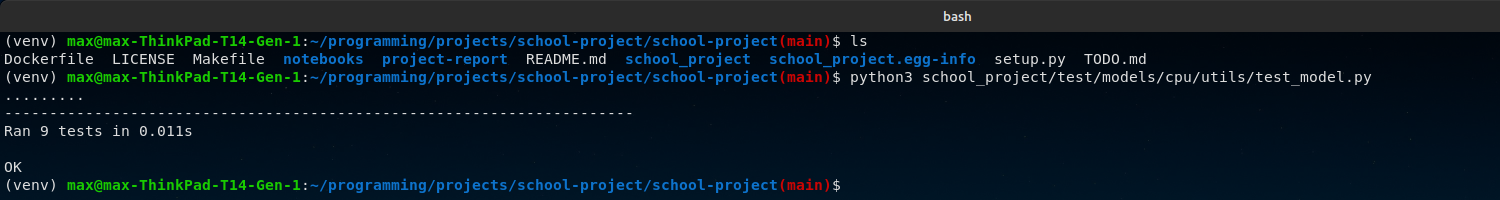
\includegraphics[width=1\textwidth]{./project-report/src/images/test-model.png}}
						\end{figure}
	
						Link to video evidence: \url{https://github.com/mcttn22/school-project/blob/main/project-report/input-validation-testing-videos.md/#test_modelpy}

				\end{itemize}
            \item test\_tools.py module:
				\begin{itemize}
					\item test\_relu:
					\begin{itemize}
						\item Description: Test ReLu output range to be greater than or equal to zero.
						\item Data Values: [-100, 0, 100]
						\item Data Type: Boundary
						\item Expected Result: The output of the ReLu transfer function should be greater than or equal to zero.
						\item Actual Result: Expected Result
						\item Test Status: Pass
					\end{itemize}
					\item test\_sigmoid:
					\begin{itemize}
						\item Description: Test sigmoid output range to be within 0-1.
						\item Data Values: [-100, 0, 100]
						\item Data Type: Boundary
						\item Expected Result: The output of Sigmoid transfer function should be between zero and one.
						\item Actual Result: Expected Result
						\item Test Status: Pass
					\end{itemize}
					\item Evidence:
                		\inputminted{python}{./school_project/test/models/cpu/utils/test_tools.py}

						\pagebreak

						\begin{figure}[h!]
						\centering
						\frame{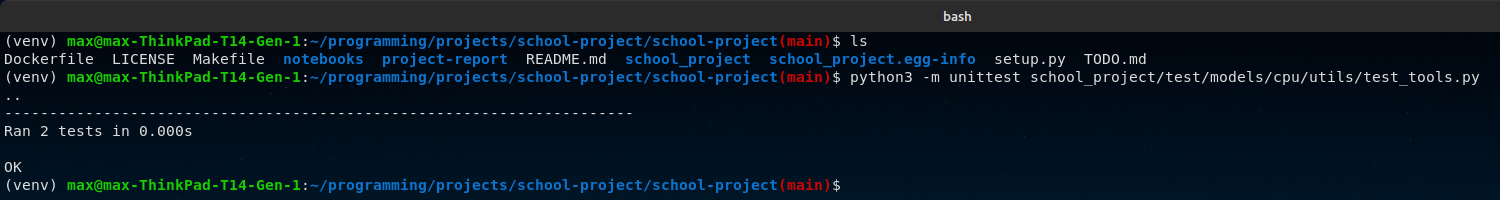
\includegraphics[width=1\textwidth]{./project-report/src/images/test-tools.png}}
						\end{figure}
	
						Link to video evidence: \url{https://github.com/mcttn22/school-project/blob/main/project-report/input-validation-testing-videos.md/#test_toolspy}
				\end{itemize}
        \end{itemize}
\end{itemize}

\subsubsection{GitHub Automated Testing}

With the following configuration programmed in the .github/workflows/tests.yml file, the unit tests are run automatically on GitHub servers after each commit that is pushed to GitHub, 
and the status of the tests (either passing or failing) can be viewed on the repository's page. This automatic testing allows for a faster workflow and allows me to identify which changes 
(commits) cause issues within the code, allowing for easier maintenance of the project.

\inputminted{yaml}{./.github/workflows/tests.yml}

\subsubsection{Docker}

I also provide a basic Dockerfile and instructions for its use in the README.md file, so that the project can be quickly run and tested in Docker containers. Below 
shows the contents of the basic Dockerfile:

\inputminted{docker}{./Dockerfile}

\end{document}
